\documentclass[12pt]{article}

\usepackage[a4paper,top=1in,bottom=1in,left=1in,right=1in]{geometry}

\usepackage[utf8]{inputenc}
\usepackage{float}
\usepackage{amsmath}
\usepackage{graphicx}
\usepackage{titlesec}
\usepackage{tcolorbox}
\usepackage{enumitem}
\usepackage{tikz}
\usepackage{tikz-timing}
\usetikzlibrary{patterns}
\usetikzlibrary{graphs}
\usetikzlibrary{graphdrawing}
\usegdlibrary{force}
\usepackage{amssymb}
\usepackage{hyperref}

\title{\bfseries Laborator Proiectare Logică 8}
\author{Sîrghe Matei}
\date{November 27, 2024}

\titleformat{\section}
  {\normalfont\Large\bfseries}{\thesection}{1em}{}
\begin{document}
\maketitle

\begin{center}
    \large{\textbf{Circuite secvențiale}}
\end{center}

\renewcommand{\arraystretch}{1}

\begin{figure}[h!]
    \begin{minipage}{0.4\textwidth}
        \begin{tikztimingtable}
            A   & LHHHHHHHHHHH \\
            B   & HLLLLLLLLLLL \\
        \end{tikztimingtable}

        \begin{tikzpicture}[overlay, shift={(0, -0.5)}]
            % X-axis label
            \node[below] at (4.5, 1) {t};
            
            % Y-axis label
            \node[rotate=90, anchor=north] at (-1, 1.5) {Semnale};
        \end{tikzpicture}
        \caption{diagrama temporală}
    \end{minipage}
    \hfill
    \begin{minipage}{0.6\textwidth}
        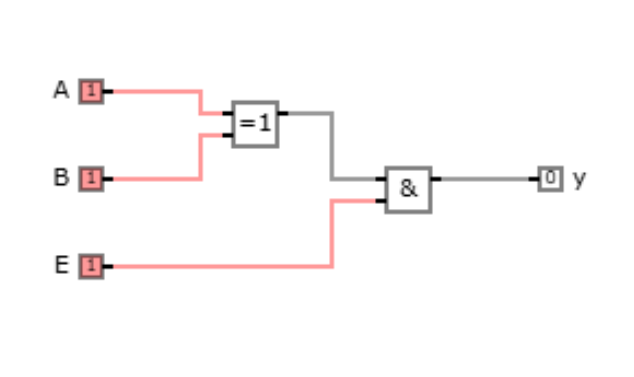
\includegraphics[scale=0.5]{Schema1.png}
    \end{minipage}
\end{figure}

\begin{figure}[h!]
    \begin{minipage}{0.45\textwidth}
        $y=\sum(3,5)=\bar{A}BE+A\bar{B}\bar{E}$\\
        $=\bar{E}(\bar{A}B+A\bar{B})=E(A\bigoplus B)$\\

        \begin{tikztimingtable}
            A   & LLLLLLLLHHHHHHHH \\
            B   & LLLLHHHHLLLLHHHH \\
            E   & LLHHLLHHLLHHLLHH \\
            $A\bigoplus B$   & LLLLHHHHHHHHLLLL \\
            y   & LLLLLLHHLLHHLLLL \\
        \end{tikztimingtable}

        \begin{tikzpicture}[overlay, shift={(0, -0.5)}]
            \node[below] at (6, 1) {t};
            
            \node[rotate=90, anchor=north] at (-1, 1.5) {Semnale};
        \end{tikzpicture}
        \caption{diagrama temporală}
    \end{minipage}
    \hfill
    \begin{minipage}{0.5\textwidth}
        \begin{tabular}{|c|c|c|c|c|}
            \hline
            A & B & E & $A\bigoplus B$ & y \\ \hline
            0 & 0 & 0 & 0 & 0 \\ \hline
            0 & 0 & 1 & 0 & 0 \\ \hline
            0 & 1 & 0 & 1 & 0 \\ \hline
            0 & 1 & 1 & 1 & 1 \\ \hline
            1 & 0 & 0 & 1 & 0 \\ \hline
            1 & 0 & 1 & 1 & 1 \\ \hline
            1 & 1 & 0 & 0 & 0 \\ \hline
            1 & 1 & 1 & 0 & 0 \\ \hline
        \end{tabular}
    \end{minipage}
\end{figure}

\newpage
\begin{center}
    \large{\textbf{Detector de front pozitiv}}
\end{center}

\begin{figure}[h!]
    \begin{minipage}{0.45\textwidth}
        $y=\bar{\bar{\bar{\bar{\bar{\bar{\bar{A}}}}}}}=\bar{A}$\\
        deoarece$ \bar{\bar{A}}=A$\\

        \begin{tikztimingtable}
            A   & LLLLLLLLHHHHHHHH \\
            $\bar{A}$   & HHHHHHHHHLLLLLLL \\
            $A\bar{A}$   & LLLLLLLLHLLLLLLL \\
        \end{tikztimingtable}

        \begin{tikzpicture}[overlay, shift={(0, -0.5)}]
            \node[below] at (6, 1) {t};
            
            \node[rotate=90, anchor=north] at (-1, 1.5) {Semnale};
        \end{tikzpicture}
        \caption{Detector de front pozitiv}
    \end{minipage}
    \hfill
    \begin{minipage}{0.5\textwidth}
        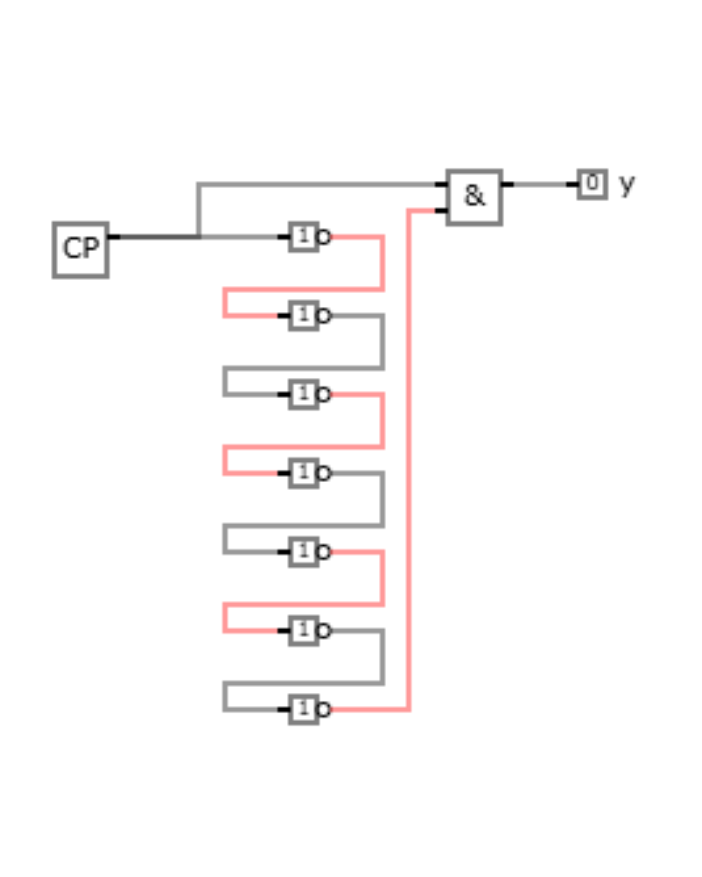
\includegraphics[scale=0.5]{Schema2.png}
    \end{minipage}
\end{figure}

\begin{center}
    \large{\textbf{Detector de front negativ}}
\end{center}

\begin{figure}[h!]
    \begin{minipage}{0.45\textwidth}
        SR-NAND
        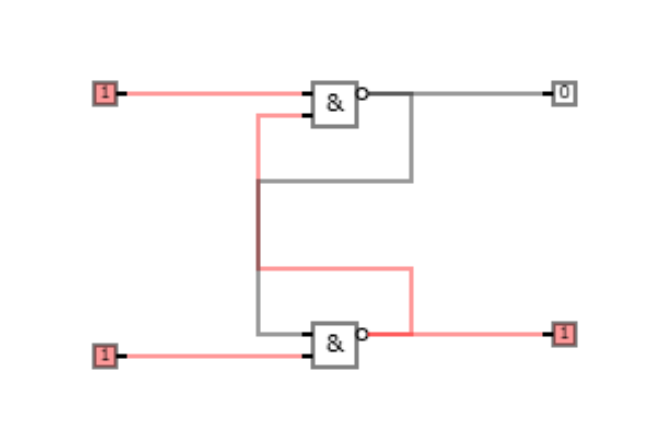
\includegraphics[scale=0.5]{Schema3.png}
    \end{minipage}
    \hfill
    \begin{minipage}{0.3\textwidth}
        \begin{tabular}{|c|c|c|c|c|}
            \hline
            A & S & Q & $\bar{Q}$ \\ \hline
            0 & 0 & 0 & 0 \\ \hline
            0 & 1 & 0 & 1 \\ \hline
            1 & 0 & 1 & 0 \\ \hline
            1 & 1 & (1 Q 0) & (0 $\bar{Q}$ 1) \\ \hline
        \end{tabular}
    \end{minipage}
\end{figure}

\newpage
SR-NOR
\begin{figure}[h!]
    \begin{minipage}{0.45\textwidth}
        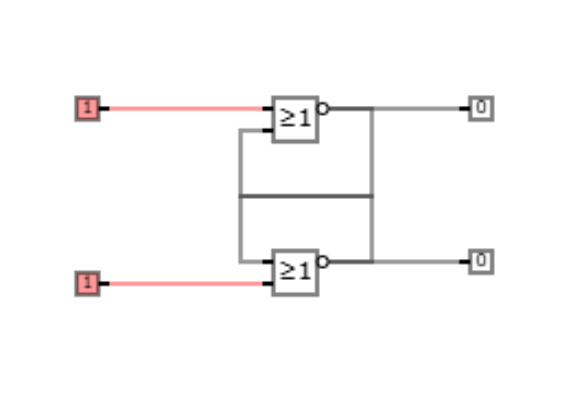
\includegraphics[scale=0.5]{Schema4.png}
    \end{minipage}
    \hfill
    \begin{minipage}{0.3\textwidth}
        \begin{tabular}{|c|c|c|c|c|}
            \hline
            A & S & Q & $\bar{Q}$ \\ \hline
            0 & 0 & (1 Q 0) & (0 $\bar{Q}$ 1) \\ \hline
            0 & 1 & 1 & 0 \\ \hline
            1 & 0 & 0 & 1 \\ \hline
            1 & 1 & 0 & 0 \\ \hline
        \end{tabular}
    \end{minipage}
\end{figure}

\begin{figure}[h!]
    \begin{minipage}{0.45\textwidth}
        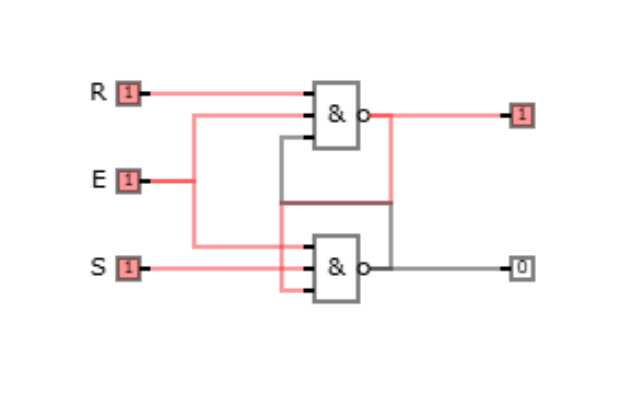
\includegraphics[scale=0.5]{Schema5.png}
    \end{minipage}
    \hfill
    \begin{minipage}{0.3\textwidth}
        \begin{tabular}{|c|c|c|c|c|}
            \hline
            E & R & S & Q & $\bar{Q}$ \\ \hline
            0 & 0 & 0 & 1 & 1 \\ \hline
            0 & 0 & 1 & 1 & 1 \\ \hline
            0 & 1 & 0 & 1 & 1 \\ \hline
            0 & 1 & 1 & 1 & 1 \\ \hline
            1 & 0 & 0 & 1 & 1 \\ \hline
            1 & 0 & 1 & 1 & 0 \\ \hline
            1 & 1 & 0 & 0 & 1 \\ \hline
            1 & 1 & 1 & Q & $\bar{Q}$ \\ \hline
        \end{tabular}
    \end{minipage}
\end{figure}

\end{document}